\documentclass[a4paper,11pt, twoside]{article}


%%%%%%%%%%%%%% Predefined packages
\usepackage{times,amsmath,eurosym, amssymb, color, graphicx}
\usepackage{booktabs, cellspace}
\usepackage[american]{babel} 
%%%%%%%%%%%%%% Packages: IF YOU NEED TO ADD A PACKAGE, PLEASE DO IT HERE:
\usepackage{cite}
%%%%%%%%%%%%%% Useful definitions
\newcommand{\R}{\mathbb R}
\newcommand{\C}{\mathbb C}
\newcommand{\F}{\mathbb F}
\newcommand{\Z}{\mathbb Z}
\newcommand{\Q}{\mathbb Q}
\newcommand{\N}{\mathbb N}

\newcommand\veczwo[2]{\left[\begin{array}{r}#1\\#2\end{array}\right]}
\newcommand\vecdrei[3]{\left[\begin{array}{r}#1\\#2\\#3\end{array}\right]}
\newcommand\vecdreic[3]{\left[\begin{array}{c}#1\\#2\\#3\end{array}\right]}
\newcommand\vecvier[4]{\left[\begin{array}{r}#1\\#2\\#3\\#4\end{array}\right]}
\newcommand\vecsechs[6]{\left[\begin{array}{r}#1\\#2\\#3\\#4\\#5\\#6\end{array}\right]}

\newcommand\matzz[4]{\left[\begin{array}{rr}#1&#2\\#3&#4\end{array}\right]}
\newcommand\matdd[9]{\left[\begin{array}{rrr}#1&#2&#3\\#4&#5&#6\\#7&#8&#9\end{array}\right]}
\newcommand\matddc[9]{\left[\begin{array}{ccc}#1&#2&#3\\#4&#5&#6\\#7&#8&#9\end{array}\right]}
%%%%%%%%%%%%%%% 



%%%%%%%%%%%%% Page layout
\topmargin-20mm
\headheight10mm
\headsep10mm
\topskip0.1mm
\hoffset-15mm
\textwidth15.5cm
\textheight22cm
\parindent0em
%\markleft{\authors}
%\markright{\shorttitle} 
\pagenumbering{arabic}
%%%%%%%%%%%%%%%%%%


\begin{document}
\thispagestyle{empty}

\hrule

$\vphantom{i}$ \\[-.25cm]

\section*{Put Your Title Here}
$\vphantom{i}\hspace{.65cm}$  \textit{and Names Here}

$\vphantom{i}$ \\[-.25cm]

\hrule

%%%%%%%%%%%%%%%%%%%%%%%%% ADD YOUR CONTRIBUTION BELOW
%%%%%%%%%%%%%%%%%%%%%%%%% USE SUBSECTION AND SUBSUBSECTION ONLY
\subsection*{Introduction}

blahblahblah

\section{Lightweight Cryptography}
% Define what lightweight cryptography is and its relevance in the field of cryptography.
The term lightweight cryptography refers to cryptographic algorithms that are designed to be secure even when operating in resource-restricted environments. These environments typically have limitations in terms of power, processing capabilities, memory, and even area/space. Lightweight cryptography aims to provide efficient and streamlined algorithms that can operate effectively in such constrained settings. It is important to note that lightweight cryptography is not a separate branch of cryptography but rather a subset of cryptographic techniques that are tailored to specific requirements.

\subsection{The Need for LWC}   % 1
% - √Discuss LWCs necessity in computing environments with limited resources like IoT devices. - chauhan2022analysis, √dutta2019lightweight, √mckay2016report
% - general terminologies and essential concepts relevant to lightweight cryptography. - ekwueme2024lightweight, √mckay2016report, √turan2021status 
% - √ Intruduce the NIST competition  More info about the competition √mckay2016report, √turan2021status
Traditional cryptographic algorithms are designed to be secure, but they are often not suitable for environments with limited resources. In recent years, there has been an increasing need for lightweight cryptographic algorithms. This need arises from the growing number of devices connected to the internet. These devices are often small and have limited capabilities.

The Internet of Things (IoT) is a network built by interconnected devices (Figure \ref{fig:IoT}). These devices gather data from their environment, such as a toaster with a temperature sensor or an actuator in a nuclear power plant, and exchange it with other devices in the network \cite{chauhan2022analysis}.

\begin{figure}[h]
    \centering
    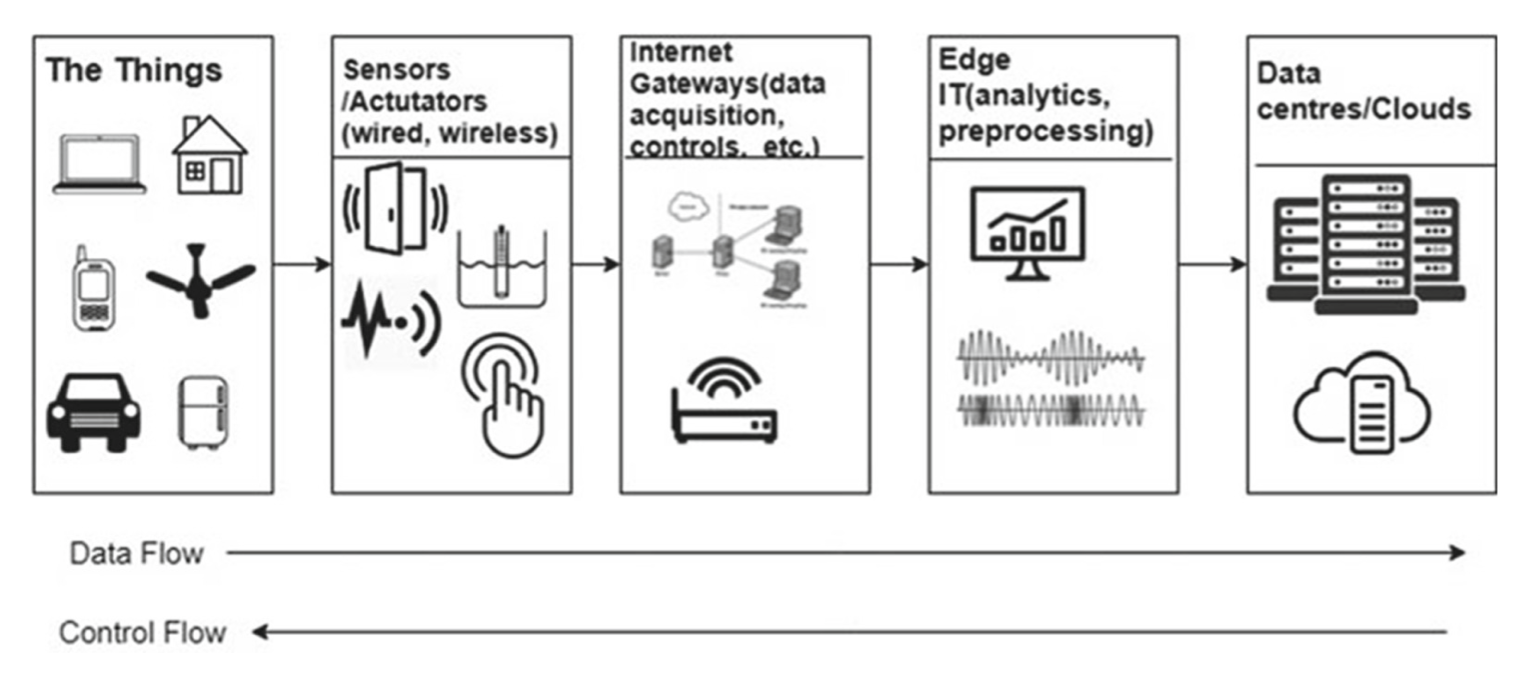
\includegraphics[width=14.0cm, height=6.0cm]{media/DesignofInternetofThings(IoT).png}
    \caption{Design of IoT}
    \label{fig:IoT}
\end{figure}

IoT devices are used in various areas and will become even more important in the future. For example, they are used in smart homes for security monitoring, smart cities for traffic control and disaster management, healthcare for patient monitoring, smart grids for energy management, and self-driving vehicles where cars can generate up to 1GB of data per second. Many of these devices operate in public and sometimes inaccessible areas, making maintenance and power supply challenging. Additionally, they are often connected over wireless networks, making them vulnerable to node tampering.

\begin{figure}[h]
    \centering
    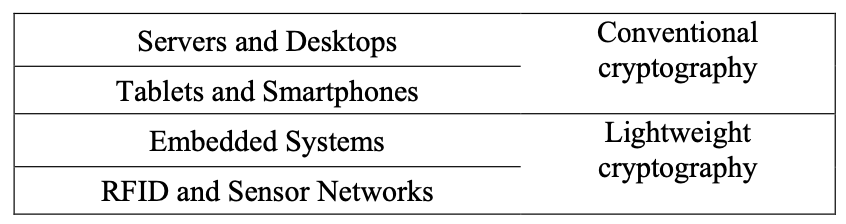
\includegraphics[width=9.0cm, height=2.5cm]{media/device_spectrum.png}
    \caption{Device Spectrum}
    \label{fig:device_spectrum}
\end{figure}

Figure \ref{fig:device_spectrum} provides a rough separation of devices and their cryptographic needs. More specifically, targeted devices can range from microcontrollers with 32-bit down to 4-bit CPUs. In these cases, the narrow data path and limited instruction set of the CPU architecture pose significant constraints. Executing complex cryptographic algorithms on such devices requires many more cycles, further slowing down the process due to potential battery constraints. Additionally, some controllers have as little as 16 bytes of RAM, while RFID devices are even more constrained \cite{mckay2016report}. Therefore, it is important to have cryptographic algorithms that are secure and do not require excessive resources \cite{IOTMarkets} \cite{dhanda2020lightweight}.

\subsubsection{NIST's Endeavor to Standardize LWC}
While the National Institute of Standards and Technology (NIST) has standardized secure algorithms like AES in the past, these algorithms are not suitable for use in IoT due to the diversity, scalability, and constantly changing nature of these devices \cite{ekwueme2024lightweight}. However, NIST initiated a project in 2015 to standardize lightweight cryptographic algorithms.

In cryptography, there is always a tradeoff between performance and the required resources to complete a task at every security level.

There are specific security needs of IoT devices that must be emphasized to have a better understanding of their requirements. These needs include:

\begin{itemize}
    \setlength{\itemsep}{-5pt}
    \item \textbf{Confidentiality}: Only authorized users or systems should have access to the devices or the network.
    \item \textbf{Availability}: The required data should be available even when multiple simultaneous connections are established.
    \item \textbf{Integrity}: Manipulation of the data should be avoided.
    \item \textbf{Authentication}: Authentication is the process of verifying the identity of a user or device. Due to the diverse range of devices and protocols in IoT networks, achieving authentication and security can be challenging \cite{dutta2019lightweight} \cite{dhanda2020lightweight}.
\end{itemize}

Further, the metrics used to define the requirements for the process of selecting lightweight algorithms are as follows:

\begin{itemize}
    \setlength{\itemsep}{-5pt}
    \item \textbf{Security}: The security of a cipher can be described as its resistance against multiple types of attacks. The security requirements include the following:
        \begin{itemize}
            \item The key size is at least 128 bits.
            \item The limits on the input sizes are at least $2^{50} - 1$ bytes.
            \item Any nonce-respecting attack on the AEAD with a 128-bit key requires at least 2112 time complexity on a classical computer in the single-key setting.
            \item Any attack on the hash function variants requires at least 2112 time complexity on a classical computer (if applicable).
        \end{itemize}
    \item \textbf{Energy consumption}: Many IoT devices run on batteries, so it is important to minimize power consumption to ensure they can complete their tasks.
    \item \textbf{Latency}: Latency is the time it takes between starting the encryption process and producing the ciphertext. Minimizing latency is crucial for fast-running systems like interconnected cars.
    \item \textbf{Throughput}: Throughput (Kbps) can be thought of as the performance that describes the frequency at which new outputs are generated, which should be in a moderate scale for these devices.
    \item \textbf{Chip Area}: This is a hardware-specific metric and describes the area of a chip implementation measured in gate equivalence (GE) in µm2. The need for area and the consumption of power can be correlated. Consequently, a smaller implementation area can reduce power consumption.
    \item \textbf{Memory Usage}: Efficient memory usage is relevant for software applications to ensure optimal performance and resource utilization. Minimizing the amount of memory required for data storage and manipulation can reduce costs and improve scalability \cite{mckay2016report}.
    \item \textbf{Efficiency}: Efficiency is the ratio between performance and resource demands. Hardware efficiency = Throughput / physical memory and Software Efficiency = Throughput / (Code Size [KB] = algorithm size).
\end{itemize}

\begin{figure}[h]
    \centering
    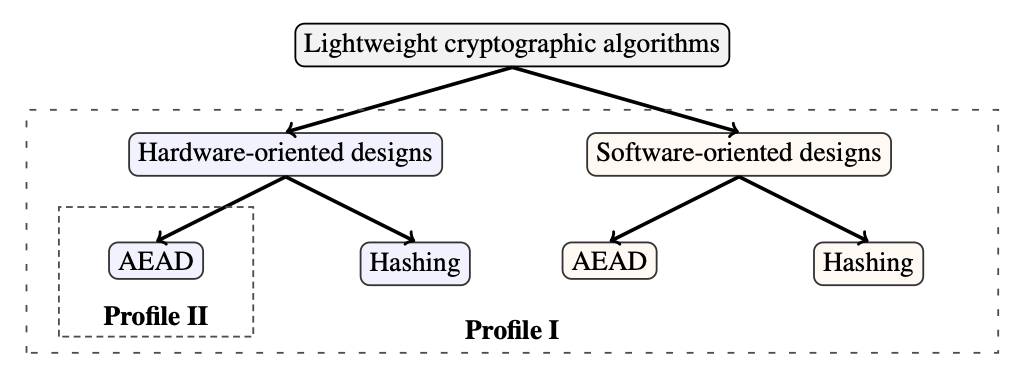
\includegraphics[width=9.0cm, height=3.5cm]{media/profiles.png}
    \caption{Profles for lightweight cryptography applications}
    \label{fig:profiles}
\end{figure}

To better understand the different needs and define the expectations of lightweight cryptography, NIST conducted a questionnaire among groups with an interest in the application of LWC. Based on the responses received, NIST created profiles that represent the requirements of these algorithms, which are influenced by the hardware and application areas where these algorithms are needed. The results of this questionnaire led to the creation of two profiles: Profile 1, which focuses on AEAD (Authenticated Encryption with Associated Data) and hashing for constrained software and hardware environments, and Profile 2, which focuses on AEAD for constrained hardware environments Figure \ref{fig:profiles}. These profiles serve as guidelines for the development and evaluation of lightweight cryptographic algorithms \cite{mckay2016report}.

\subsection{Security Issues Addressed by Lightweight Cryptography}   % 2
% -  specific security challenges that lightweight cryptography aims to solve, such as power constraints, processing capabilities, and memory limitations. - √dhanda2020lightweight, √ekwueme2024lightweight, √pammu2016interceptive
% - explain how traditional cryptographic techniques are unsuitable for such environments and highlight the differences. - Ldhanda2020lightweight: p.6
As mentioned above, IoT devices are openly deployed and process and transmit sensitive and important data, making them targets of high interest for various attacks. Some of these attacks include denial of service (DoS) attacks, where the goal is to shut down the targeted system, such as a server, by overwhelming it with a high volume of data. In addition, IoT devices with weak built-in security and low computing power, such as CCTV cameras and baby monitoring devices, can be injected with malware and used to execute distributed denial of service (DDoS) attacks on servers \cite{mckay2016report} \cite{salim2020distributed}. These attacks can have severe consequences, especially in critical applications like e-Health, where a service outage could be life-threatening, or in smart cities, where an attack could disrupt the functioning of an entire city \cite{dhanda2020lightweight}.

Crucial attacks on IoT devices include:

\begin{itemize}
    \item Exhaustive key assault attack: This attack tries to determine the key by attempting as many keys as possible, also known as a brute force attack. Lightweight cryptography needs to ensure that it can withstand brute force attacks despite using shorter key lengths that are suitable for small devices. Cryptographic systems that use a key length of $2^{128}$ and higher are considered secure enough, as the theoretical attack limit is less than $2^{128}$ with current technology.
    \item Table lookup attack: This attack involves pre-computing the ciphertexts for all possible keys of a given length. It poses a risk for devices that use predictable or not complex enough keys.
    \item Differential attacks: These attacks are successful when changes in plaintext result in predictable changes in ciphertext \cite{ekwueme2024lightweight}.
    \item One quite interesting attack is the Algebraic Fault Attack (AFA), in this case attackers induce faults into the encryption process and use algebraic techniques to analyze these faults and ultimately recover the key. Firstly these faults are induced during the encryption process by manipulating physical conditions like voltage, temperature, or clock frequency of the device. Secondly the corrupted outputs are collected. Those outputs are influenced by the specific induced faults and differ from the expected results. Thirdly a set of algebraic equations are formulated based on the differences between the expected outputs and the faulty outputs. Those equations represent the relationship between the cryptographic key (or other secret data), the input, the faulty output, and the nature of the fault. The next step is to solve these algebraic equations for the unknowns, which typically include the secret cryptographic keys. The process of solving can be computationally intensive and involve advanced algebraic computations and special software tools. Lastly if the equations are solved, sensitive information and the key can be extracted and used to decrypt other messages and data that have been secured with the extracted key. Since lightweight block ciphers have simpler algebraic structures than ciphers, the induced faults have a bigger impact on them and the equations can be solved easier, thus this attack can be a significant security risk. Some alarming results are for example that if the attacker has knowledge over 24 key bits and alters two bits in the 13-th round, DES can be broken with a single fault injection in 0.01 hour resulting in 10x the speed of a brute force attack \cite{zhang2016framework}.
    \item A case particularly relevant in IoT applications is the Side Channel Attack (SCA). SCAs do not exploit the algorithm itself but the physical leakages from a cryptographic device during its normal operation. These leakages can be power consumption, electromagnetic emissions, timing information, etc. An experiment on how this is done can be seen in Figure \ref{fig:em_measurment}. Here the electro magnetic (EM) signal of two Arduino microcontrollers, which are implementing AES-128 algorithm is measured \cite{pammu2016interceptive}.
    
        \begin{figure}[h]
            \centering
            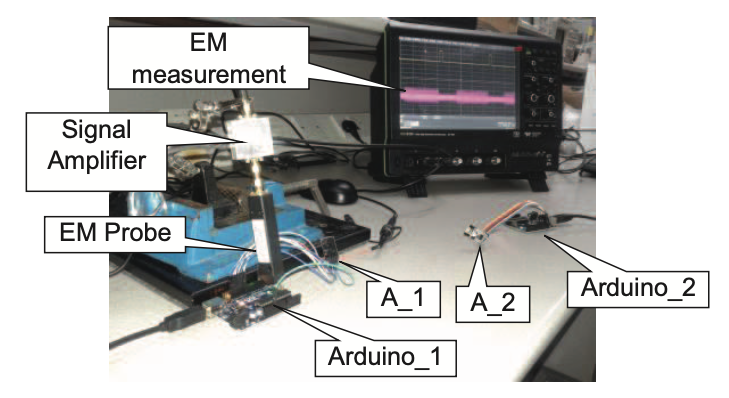
\includegraphics[width=10cm, height=4cm]{media/em_measurment.png}
            \caption{EM measurement of AES-128 based Arduino implementation}
            \label{fig:em_measurment}
        \end{figure}

    Since these devices have limited computing power, the operations they perform, such as multiplications and additions, can be analyzed. In contrast, PCs with high computational capabilities are not as easily analyzed for patterns.
    \end{itemize}



\subsection{Mechanisms and Functionality}   % 3
% - describe the general mechanisms employed in lightweight cryptography, emphasizing streamlined algorithms and efficient implementations. - khudoykulov2022comparison, chauhan2022analysis, dhanda2020lightweight
% - Discuss common models and methods used, highlighting both advantages and disadvantages. dhanda2020lightweight, mckay2016report


\subsection{Unaddressed Needs and Introduction to Ascon}   % 4
% - Nist requirements for LWC algorithms, mckay2016report, turan2021status
% - / the limitations or needs that were unaddressed by previous lightweight cryptographic approaches. dhanda2020lightweight
% - Transition into how Ascon addresses these gaps, setting the stage for the detailed exploration of Ascon in the subsequent sections. - turan2021status



\bibliographystyle{IEEEtran}
\bibliography{references}
\end{document}
